\chapter{Metodología}
\label{chapter:metodologia}

Conforme a los objetivos planteados en la sección~\ref{intro_objetivos} se
presentan las colecciones y algoritmos que serán evaluados junto con los
escenarios de flujos continuos diseñados a este fin. En la
sección~\ref{generacion_flujos_sinteticos} se describen las técnicas presentadas
en este trabajo: una variante a un método de generación de flujos continuos
(subsección~\ref{generacion_flujos_sinteticos}) y un algoritmo novedoso de
clasificación \acrshort{mll} basada en ensambles
(subsección~\ref{tecnica_algoritmo_ensamble}). Finalmente, en la
sección~\ref{materiales_y_metodos} se describen los materiales y métodos
seleccionados para llevar a cabo los experimentos.

En primer lugar, se seleccionaron tres colecciones de datos de multi-etiquetas
que han sido puntos de referencia en otros trabajos de investigación. Cada una
de ellas fue transformada en un flujo continuo de datos que cumple con las
características presentadas en la sección~\ref{stream_caracteristicas}. A su
vez, se generaron instancias sintéticas que sean fieles a las cualidades
subyacentes de los datos originales.  Para ello, se diseñó un algoritmo basado
en la implementación
de~\citeauthor{read_multi-label_2008}~\cite{read_multi-label_2008}, y que además
hace uso de un vector de probabilidades a priori de cada etiqueta, junto con una
matriz de probabilidades condicionales entre pares de etiqueta, para respetar
sus interdependencias subyacentes y así obtener datos más próximos a los
originales. Adicionalmente, se realizó un estudio de los \textit{streamings}
sintéticos generados en búsqueda de conocer su grado de proximidad o cercanía
con respecto a sus respectivas colecciones originales. El estudio incluye una
comparativa entre el método de~\citeauthor{read_multi-label_2008} y la
alternativa aquí presentada. En la sección~\ref{generacion_flujos_sinteticos} se
entrará más en detalle al respecto.

En segundo término, se diseñó e implementó el ambiente de pruebas para realizar
el entrenamiento y evaluación de los algoritmos de \acrshort{mll} en ambientes
de \textit{streaming}. La etapa de entrenamiento se llevó a cabo con algoritmos
de clasificación multi-etiquetas que han sido adaptados a ambientes de flujos
continuos para hacer frente a las cualidades incrementales inherentes a este
contexto. Se seleccionaron algoritmos de la familia de \comillas{Transformación
	del problema} y \comillas{Adaptación del algoritmo}, junto con soluciones de
ensamble, a fines explorativos y para extender el conocimiento sobre sus
fortalezas y debilidades.  Los experimentos se realizan con algoritmos
implementados en el lenguaje de programación
Python~\footnote{\url{https://www.python.org/}}.  Aquellos que no soportan datos
de múltiples etiquetas han sido acondicionados a ese fin de acuerdo al diseño
especificado en la literatura y consultando las respectivas implementaciones en
otros lenguajes de programación, de hallarse estas disponibles al público. Todos
los algoritmos utilizados para las pruebas se encuentran disponibles al
público~\footnote{\url{https://github.com/Juancard/scikit-multiflow/}}.

De manera complementaria, se diseñó una solución de ensambles llamada
\acrfull{efmp}, basada en las implementaciones existentes. La misma usa como
clasificadores base tres algoritmos de \acrshort{mll} diferentes, que se
mantienen fijos, es decir, el número de clasificadores base no cambia durante el
entrenamiento. La diversidad está dada por los algoritmos miembros del ensamble
y también por sus rendimientos previos. Con respecto a esto, el ensamble
mantiene un vector de pesos para cada clasificador base que guarda el valor de
ponderación de un miembro con respecto a una etiqueta. En caso de que una
instancia sea mal clasificada, se penaliza el clasificador y se reduce dicho
valor de ponderación. La combinación de los votos se lleva a cabo por votación
por mayoría ponderada, teniendo en cuenta la predicción realizada por cada
miembro y su respectivo vector de pesos. La implementación se basa en la
presentada por~\citeauthor{kolter_dynamic_2007}~\cite{kolter_dynamic_2007}
descritaa en la sección~\ref{ensambles_mll}. Los autores también ponderan los
clasificadores, pero usan un único algoritmo para generar los $n$ clasificadores
base, y no contemplan problemas de múltiples etiquetas. Los experimentos se
realizan con dos versiones, una de ellas se entrena con todas las instancias del
subconjunto de entrenamiento y la otra tomando muestreos siguiendo la
distribución de \textit{poisson}, tal como se realiza para ensambles del tipo de
\textit{Oza bagging}~\cite{oza_online_2005}. En la
sección~\ref{tecnica_algoritmo_ensamble} se describirá en detalle esta solución
de ensambles. La implementación del algoritmo y sus variaciones también se
encuentra disponible al
público~\footnote{\url{https://github.com/Juancard/multi-label-classification-on-data-streamings}}.

Para la etapa de evaluación se siguió la estrategia
\comillas{\textit{Prequential}}, descrita en la sección~\ref{stream_evaluacion}.
Para cada algoritmo se genera un modelo para entrenar y predecir sobre las tres
colecciones de datos seleccionadas. Cada modelo realiza primero la predicción
sobre una instancia sin sus etiquetas, luego se entrena con las etiquetas reales
y se actualizan las métricas con las etiquetas inferidas y reales. Se aplicaron
métricas de \acrshort{mll} basadas en etiquetas, en ejemplos, y además se mide
la eficiencia de los modelos en términos de velocidad y espacio de
almacenamiento. Con los resultados obtenidos, se realizó un estudio comparativo
del rendimiento por cada colección, y se analiza cuáles son los modelos que
mejores resultados han obtenido para cada caso.

El marco metodológico de este proyecto se ajusta a los procedimientos efectuados
previamente por otros investigadores de la
literatura~\cite{osojnik_multi-label_2017, sousa_multi-label_2018,
	buyukcakir_novel_2018, zheng_survey_2020, read_scalable_2012}. Con ello se ha
buscado expandir el conocimiento empírico de los algoritmos al mismo tiempo que
proporcionar nuevos estudios que sean contrastables con los ya existentes.
Dichos estudios también incluyen el análisis de las evaluaciones realizadas por
el ensamble \acrshort{efmp} y su comparativa de rendimiento con respecto a otros
algoritmos conocidos del campo. En cuanto a la generación sintética de datos,
este proyecto siguió la línea de investigación presentada
por~\citeauthor{read_generating_2009}. A este respecto, se generaron
\textit{streams} sintéticos bajo el método presentado por dichos autores y bajo
el método aquí presentado. Con dichos \textit{streams} se realizó un análisis de
las cualidades y fenómenos hallados, siguiendo las directivas presentadas en su
escrito~\cite{read_generating_2009}. Se destaca también el trabajo
de~\citeauthor{read_scalable_2012}~\cite{read_scalable_2012}, quienes analizan
algoritmos multi-etiquetas con flujos reales y sintéticos, pero a diferencia de
este trabajo, generan instancias sintéticas para colecciones nuevas y sin
basarse en colecciones reales específicas. La implementación del generador que
usaron en sus experimentos se encuentra disponible al
público~\cite{read_moa_2012} y ha sido el punto de partida para desarrollar la
técnica aquí propuesta.  \citeauthor{buyukcakir_novel_2018}, por su parte, no
generan flujos sintéticos, pero conducen experimentos similares en lo que
respecta a la evaluación de algoritmos, poniendo el foco en modelos de
ensambles.  La implementación de sus experimentos también ha sido liberada al
público~\footnote{\url{https://github.com/abuyukcakir/gooweml}} y fue uno de los
modelos a tener en cuenta en el análisis de rendimiento de la solución de
ensambles \acrshort{efmp}. Otros puntos de referencia para estudiar el algoritmo
aquí presentado fueron los modelos iSOUP-MT e iSOUP-RT
de~\citeauthor{osojnik_multi-label_2017}~\cite{osojnik_multi-label_2017} y
ML-SAM-kNN
de~\citeauthor{roseberry_multi-label_2018}~\cite{roseberry_multi-label_2018}.

\section{Técnicas Propuestas}
\label{tecnicas_propuestas}

En esta sección se describen dos técnicas implementadas para este trabajo: un
generador de instancias sintéticas para flujos continuos de datos y el diseño de
una solución de ensambles para realizar clasificaciones.

\subsection{Generación de Flujos Sintéticos}
\label{generacion_flujos_sinteticos}

El generador presentado es un algoritmo que emplea técnicas probabilísticas para
hallar dependencias entre etiquetas y reproducirlas en las nuevas instancias. La
existencia de interdependencias entre etiquetas ha sido explorada reiteradas
veces en la literatura~\cite{tsoumakas_multi-label_2007, read_multi-label_2008}
y se ha demostrado que existen dependencias condicionales e incondicionales,
esto es, etiquetas que dependen entre sí dado uno o más atributos de una
instancia (dependencia condicional), y etiquetas cuya dependencia existe para
todo el conjunto de instancias (dependencia incondicional). Estas dos cualidades
son directamente extraídas de las colecciones reales y a partir de ellas se
genera el espacio de atributos y etiquetas que, al fusionarse, constituyen la
instancia sintética.

La dependencia incondicional parte de la idea de que hay etiquetas que se
activan en conjunto con frecuencia y otras que son mutuamente excluyentes. Véase
el caso de las etiquetas \comillas{\texttt{Ficción}} y \comillas{\texttt{No
		Ficción}}, por ejemplo, que son excluyentes en el dominio de géneros literarios.
Para capturar esta relación se acude al concepto de probabilidad a priori y
probabilidad condicional de etiquetas. La probabilidad a priori de una etiqueta
es obtenida a partir de observar su frecuencia relativa en la colección y
normalizarla por la cardinalidad de etiquetas. La frecuencia relativa se formula
de la manera tradicional:

\begin{equation}
	FrecRelE_{j} = \frac{1}{m} \sum_{i=1}^{m} y_{i,j}
\end{equation}

La normalización toma en cuenta el valor de cardinalidad de etiquetas del
conjunto de datos, esto bajo la recomendación de los autores del trabajo de
referencia~\cite{read_scalable_2012}.

\begin{equation}
	NormCardE = \frac{1}{CardE} \sum_{j=1}^{q} FrecRelE_{j}
\end{equation}

Donde $CardE$ se define tal como en~\ref{eq:mll_card}, esto es:

\begin{equation}
	CardE(D) = \frac{1}{m} \sum_{i=1}^{m} \left\|Y_{i}\right\|
\end{equation}

Luego, la probabilidad a priori de la etiqueta $j$ se expresa de la forma:

\begin{equation}
	P(E_{j}) =\min{(1, \frac{FrecRelE_{j}}{NormCardE})}
\end{equation}

El resultado es un vector $[P(E_{1}), P(E_{2}),\dots, P(E_{q})]$.

A partir de $P(E_{j})$ se puede calcular la matriz condicional $\theta$ sobre
los pares de etiquetas, esto es, $\theta_{j,k} = P(Y_{j} = 1 \mid Y_{k} = 1)$,
donde  $1 \leq j \leq L$ y $1 \leq k \leq L$ con $j \neq k$. Con el vector de
probabilidades a priori y extrayendo las co-ocurrencias de cada par de etiquetas
en toda la colección, es posible obtener cada valor de la matriz $\theta$,
aplicando la probabilidad condicional:

\begin{equation}
	P(Y_{j} = 1 \mid Y_{k} = 1) = \frac{P(Y_{k} = 1 \cap Y_{j} = 1)}{P(Y_{k})}
\end{equation}

Luego, la dependencia entre etiquetas es modelada como la distribución conjunta:

\begin{equation}
	\label{eq:syn_joint}
	p_{\theta}(y) = P(y_{1}) \prod_{j=2}^q P(y_{j} \mid y_{j-1})
\end{equation}

Posteriormente, se realiza la generación del conjunto de etiquetas para la
instancia sintética. El algoritmo~\ref{alg:generar_etiquetas} muestra las
instrucciones ejecutadas para concretar esta tarea. Cabe aclarar que $sample()$
retorna un índice de etiqueta de acuerdo a una función de masa de probabilidad
basada en las probabilidades a priori, y $random()$ produce un número aleatorio
de distribución uniforme.

% textidote: ignore begin
\begin{center}
	\begin{algorithm}[H]
		\label{alg:generar_etiquetas}
		\SetAlgoLined
		\DontPrintSemicolon
		\KwIn{
			$q$:  Número de etiquetas de la colección,
			$p$: vector de probabilidades a priori,
			$p_{\theta}(y)$: función definida en fórmula~\ref{eq:syn_joint}
		}
		\KwOut{$y$: las etiquetas generadas.}
		$y \gets \emptyset_{q}$\;
		$j \gets sample(p)$\;
		$y_{j} \gets 1$\;
		$i \gets 0$ \;
		\While{$i < q$}{
			\lIf{$i = j$}{$\Continue$}
			$y^{\prime} \gets y$\;
			$y^{\prime}_{i} \gets 1$\;
			\lIf{$p_{\theta}(y^{\prime}) > random()$}{$y \gets y^{\prime}$ }
			$i \gets i+1$\;
		}
		\caption{Algoritmo de generación del conjunto de etiquetas para una instancia
			sintética.}
	\end{algorithm}
\end{center}
% textidote: ignore end

Una vez generado el conjunto de etiquetas resta generar los valores de atributos
para la instancia. Para ello se retoma el concepto ya mencionado de
\comillas{Dependencia Condicional}, para conocer en qué medida la presencia de
un atributo activa una o más etiquetas en la instancia, o expresado en términos
formales, hallar el término $P(y|x)$ tal que:

\begin{equation}
	P(y|x) = P(x|y)P(y)
\end{equation}

Como el cálculo de la probabilidad conjunta es altamente complejo se define una
función de mapeo $\zeta[a] \mapsto y_{a}$, donde $y_{a}$ es la combinación de
etiquetas más probable para el atributo $a$.  La función $\theta$ se obtiene a
través de muestreos sucesivos del generador de etiquetas, y guardando las $A$
combinaciones más frecuentes, siendo el número total de atributos. Al mismo
tiempo, el vector $x$ candidato es obtenido usando un generador binario tal como
los descritos en la sección~\ref{stream_syn}. El
algoritmo~\ref{alg:generar_atributos} muestra un pseudocódigo de cómo se
completa el proceso. Notar que el generador binario $g$ produce dos vectores de
atributos candidatos, uno por cada clase, luego si la combinación de etiquetas
para el atributo $a$ es un subconjunto de las etiquetas generadas se toma el
valor de esa posición de atributo en el vector de atributos positivos. Caso
contrario, se toma del vector de negativos.

Finalmente, la instancia sintética se forma a partir de la salida de ambos
algoritmos, siendo de la forma $(x, y)$. Este proceso será repetido para cada
instancia que se solicite al generador a fin de generar el flujo sintético para
la colección dada. El objetivo es obtener colecciones sintéticas que se asemejen
a datos del mundo real, por lo tanto, la evaluación de los resultados se hará
mediante un análisis de sus cualidades en relación con fenómenos hallados en
datos reales (ver sección~\ref{mll_fenomenos}), y se contrastan los datos
generados en este marco contra los producidos en el trabajo de referencia.

La configuración y parametrización de los flujos continuos generados en el marco
de este trabajo serán descritos en detalle en el
capitulo~\ref{chapter:experimentos}:\comillas{~\nameref{chapter:experimentos}}.

% textidote: ignore begin
\begin{center}
	\begin{algorithm}[H]
		\label{alg:generar_atributos}
		\SetAlgoLined
		\DontPrintSemicolon
		\KwIn{
			$A$:  Número de atributos de la colección,
			$g$: Generador de atributos,
			$\zeta$: Función de mapeo.
		}
		\KwOut{$x$: El vector de atributos generado.}
		$x \gets \emptyset_{A}$\;
		$positivos \gets g(1)$ \;
		$negativos \gets g(0)$ \;
		$i \gets 0$ \;
		\While{$i < A$}{
			\uIf{$\exists q : \zeta[a] \subseteq y_{q}$}{
				$x_{i} \gets positivos_{i}$ \;
			}
			\Else{
				$x_{i} \gets negativos_{i}$ \;
			}
			$i \gets i+1$ \;
		}
		\caption{Algoritmo de generación del conjunto de atributos para una
			instancia sintética.}
	\end{algorithm}
\end{center}
% textidote: ignore end

\subsection{Algoritmo de Ensamble}
\label{tecnica_algoritmo_ensamble}

\acrfull{efmp} es una estrategia de ensamble en ambientes de flujos continuos
que pondera a los clasificadores base de acuerdo a su rendimiento y ajusta los
pesos en cada predicción, a fin de optimizar la exactitud y eficiencia de la
respuesta, y al mismo tiempo mantenerse actualizado frente a los cambios de
concepto. Además, es un ensamble que permite definir clasificadores base
modelados a partir de algoritmos de clasificación diferentes para explotar la
variabilidad en los mismos. La técnica de ponderación se basa en la presentada
por \citeauthor{kolter_dynamic_2007} para la estrategia \textit{\acrlong{dwm}}
(\acrshort{dwm})~\cite{kolter_dynamic_2007} y fue ajustada para soportar datos
de múltiples etiquetas. Otra de las cualidades del ensamble \acrshort{dwm} es
que agrega y elimina clasificadores base dinámicamente de acuerdo a su
ponderación. Sin embargo, el costo computacional acarreado es notorio y los
nuevos modelos añadidos son de un mismo tipo y no permite variarlos.  En
consecuencia, se presenta la estrategia \acrshort{efmp} como posible alternativa
junto con una variación del mismo, \acrshort{efmp2}, que muestrea instancias
según la distribución \textit{poisson}. A continuación, se describen ambas
técnicas en detalle.

\acrshort{efmp} mantiene un conjunto fijo de $m$ clasificadores base, cada uno
con un vector de pesos $W_{k} = [w_{0}, w_{1}, \dots, w_{q}]$, donde $1 \leq k
	\leq m$ y $w_{k,j}$ representa el peso del clasificador $k$ para la etiqueta
$j$. En el entrenamiento del modelo se reciben $n$ instancias donde
$n=\left\|D\right\|$ para la estrategia simple. Además, se definen los parámetros
$p$, que es la cantidad de instancias observadas entre actualizaciones de los
pesos, y $\beta$, que representa el factor en el que se decrece el peso
$w_{k,j}$ ante cada clasificación errónea. $\beta$ es un valor definido en el
dominio $0 \leq \beta \leq 1$ y toma el valor $0.5$ por defecto. Todos los pesos
son inicializados en 1.

El proceso de aprendizaje se lleva a cabo de la siguiente manera: al arribar una
instancia $i$, \acrshort{efmp} se la asigna a cada uno de los $m$
clasificadores. En primer lugar, se realiza la actualización de pesos y si un
clasificador $C_{k}$ no predice correctamente una etiqueta $j$, su peso
$w_{k,j}$ será multiplicado por el factor $\beta$. Luego, se entrena cada
clasificador con la instancia nueva y se repite el procedimiento con la
siguiente. El parámetro $p$ es usado durante esta etapa y determina los períodos
entre los cuales no se deben actualizar los pesos. Una vez completado un período
se normalizan los pesos de manera tal que el máximo peso entre etiquetas es uno.
El algoritmo~\ref{alg:entrenamiento_efmp} presenta el pseudocódigo de este
proceso en detalle.

% textidote: ignore begin
\begin{center}
	\begin{algorithm}[H]
		\label{alg:entrenamiento_efmp}
		\SetAlgoLined
		\DontPrintSemicolon
		\KwIn{
			$\{X,Y\}$: Conjunto de entrenamiento,
			$n$: Número de instancias de entrenamiento,
			$q$: Número de etiquetas,
			$\beta$: Factor de decrecimiento de los pesos,
			$p$: Período entre actualizaciones de los pesos,
			$C$: Clasificadores base,
			$W$: Pesos de los clasificadores
		}
		$i \gets 0$ \;
		$m \gets \left\|C\right\|$ \;
		\While{$i < n$}{
			\If{$i \bmod p = 0$}{
				$k \gets 0$ \;
				\While{$k < m$}{
					$y_{i} \gets predecir(C_{k}, X_{i})$ \;
					$j \gets 0$ \;
					\While{$j < q $}{
						\If{$y_{i, j} \neq Y_{i,j}$}{
							$W_{k,j} \gets \beta * W_{k,j}$ \;
						}
						$j \gets j+1$ \;
					}
					$k \gets k+1$\;
				}
				$W \gets escalarPesos(W)$ \;
			}
			$k \gets 0$ \;
			\While{$k < m$}{
				$entrenar(C_{k}, X_{i}, Y_{i})$ \;
				$k \gets k+1$\;
			}
			$i \gets i+1$\;
		}
		\caption{Algoritmo de entrenamiento y ajuste de pesos para \acrfull{efmp}}
	\end{algorithm}
\end{center}
% textidote: ignore end

Durante la etapa de predicción cada clasificador retorna su voto $v_{i,j,k}$ y
el ensamble realiza la combinación computando la suma ponderada para cada
etiqueta. La ecuación es la siguiente:

\begin{equation}
	y_{i,j} = \frac{1}{\sum_{k=1}^{m} w_{j,k}} \sum_{k=1}^{m} v_{i,j,k} *
	w_{j,k}
\end{equation}

Las etiquetas cuyo valor superen un umbral de $0.5$ serán activadas:

\begin{equation}
	y_{i,j} =
	\begin{cases}
		1, & \text{si}\ y_{i,j} \geq 0.5 \\
		0, & \text{de otro modo.}
	\end{cases}
\end{equation}

\acrshort{efmp2} introduce una única variación, durante el entrenamiento. Cuando
arriba una instancia $i$, cada uno de los clasificadores base entrena el modelo
$Poisson(1)$ veces con dicha instancia. Esta técnica es conocida como
\textit{online bagging} y se ha probado que se aproxima a la estrategia
tradicional de \textit{bagging} en \textit{batch}, cuando se entrena con
ejemplos de distribución similar~\cite{oza_online_2005}.

En el próximo capítulo se retoma este algoritmo para profundizar sobre la
configuración experimental y el ambiente de pruebas en el que fueron llevadas a
cabo las fases de entrenamiento y evaluación de este modelo, y de los demás
algoritmos de referencia.

\section{Materiales y Métodos}
\label{materiales_y_metodos}

En esta sección se presentan y caracterizan las colecciones de datos utilizadas
en las pruebas y luego se detalla el ambiente en el cual se ejecutaron los
experimentos, incluyendo información sobre el hardware y software empleado. Una
vez hecho esto, se listan los algoritmos seleccionados para las pruebas, junto
con la bibliografía emparentada y la configuración particular de cada uno de
ellos, y las métricas de evaluación adoptadas y con las cuales se comparan los
modelos.

\subsection{Colecciones}

\begin{table}[htbp]
	\centering
	\begin{tabular}{llrrrrr}
	\toprule
	Nombre    & Dominio & N     & A    & L   & LC    & LD    \\
	\midrule
	20ng      & Texto   & 19300 & 1006 & 20  & 1,029 & 0,051 \\
	Enron     & Texto   & 1702  & 1001 & 53  & 3,378 & 0,064 \\
	Mediamill & Video   & 43907 & 120  & 101 & 4,376 & 0,043 \\
	\bottomrule
\end{tabular}

	\caption[Colecciones multi-etiquetas y sus características.]{Colecciones
		multi-etiquetas y sus características. N:\@ número de
		instancias; A:\@ número de atributos; L:\@ número de etiquetas; LC:\@ cardinalidad
		de etiquetas; LD:\@ densidad de etiquetas.}
	\label{tab:datasets}
\end{table}

Se seleccionan colecciones de datos multi-etiquetas del mundo real que han sido
aplicados previamente en la literatura para evaluar la capacidad predictiva de
los modelos de
clasificación~\cite{osojnik_multi-label_2017,read_scalable_2012,buyukcakir_novel_2018}.
La tabla~\ref{tab:datasets} enumera sus características principales, incluyendo
métricas que describen su grado de multi-etiquetado (ver
sección~\ref{mll_def_formal}). Una descripción detallada de cada una se lista a
continuación:

\begin{description}

	\item{20ng}\footnote{\url{https://www.uco.es/kdis/mllresources/}}: Es una
	      colección que consta de casi 20 mil publicaciones provenientes de grupos de
	      noticias y que abordan 20 tópicos diferentes~\cite{lang_newsweeder_1995}.
	      La colección es de texto y fue preprocesada para formar 1006 atributos
	      numéricos.

	\item{Enron}\footnote{\url{http://sourceforge.net/projects/mulan/files/datasets/enron.rar}}:
	      Es una colección de correos electrónicos seleccionados de entre los 500
	      mil generados por empleados de la compañía eléctrica \textit{Enron} y
	      filtrados durante una investigación por
	      corrupción~\cite{hutchison_enron_2004}. Su tamaño, que no supera los
	      2000 elementos, no es lo suficientemente grande para ser considerado un
	      flujo continuo voluminoso, pero sí cuenta con otras propiedades como la
	      inclusión de fechas y una evolución de los datos en el
	      tiempo~\cite{read_scalable_2012}. Las etiquetas se dividen en cuatro
	      grupos, según su género (acuerdos laborales, correos meramente
	      personales, etc.); según la información que incluyen, esto es, si el
	      correo contiene enlaces externos, adjuntos, reenvíos, etc.; según el
	      tono emocional que reflejan y según el tópico principal que abordan.

	\item{Mediamill}\footnote{\url{https://sourceforge.net/projects/mulan/files/datasets/mediamill.rar}}:
	      Es una colección generada a partir de 80 horas de video provenientes de
	      transmisiones de noticias durante noviembre de
	      2004~\cite{snoek_challenge_2006}. Se seleccionaron más de 43 mil
	      ejemplos y fue manualmente etiquetada con 101 conceptos, que pueden
	      visualizarse en la figura~\ref{fig:mediamill}.

\end{description}

\begin{figure}[htbp]
	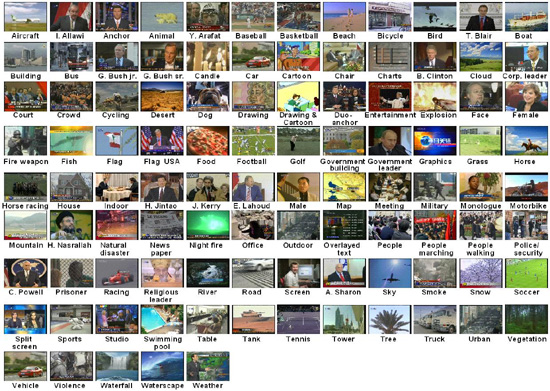
\includegraphics[width=.9\linewidth]{figures/mediamill.jpg}
	\centering
	\caption{Los 101 conceptos semánticos asociados a la colección
		Mediamill.}
	\label{fig:mediamill}
\end{figure}

Estas son solo tres de las colecciones usualmente abordadas en la literatura y
se han seleccionado con el objetivo de diversificar el análisis. Enron es una
colección de pocas instancias, pero muchas etiquetas, 20ng a la inversa, cuenta
con pocas etiquetas, pero muchas instancias; y Mediamill, finalmente, es la
colección con más instancias que hay disponible y cuenta también con un número
relativamente alto de etiquetas.

Durante la ejecución de experimentos, cada colección será convertida a un flujo
sintético. Además, se generará una versión sintética de cada una, siguiendo la
técnica descrita en la sección~\ref{generacion_flujos_sinteticos}.

\subsection{Software}

A continuación se describen las herramientas de software que fueron utilizadas
para la implementación y ejecución de los experimentos.

\begin{description}

	\item[scikit-multiflow]\footnote{\url{https://scikit-multiflow.github.io/}}
	      Es una librería disponible para el lenguaje de programación Python que
	      provee un \textit{framework} para implementar y comparar algoritmos de
	      aprendizaje automático en ambientes de flujos continuos de datos.
	      Incluye pero no se limita a problemas de clasificación
	      multi-etiquetas~\cite{montiel_scikit-multiflow_2018}.

	\item[\acrshort{moa}]\footnote{\url{https://moa.cms.waikato.ac.nz/}}
	      \acrfull{moa} es un \textit{framework} para realizar minería de datos
	      sobre flujos continuos de datos, implementada en Java y de código libre.
	      Incluye algoritmos de evaluación y de aprendizaje automático como
	      clasificadores, regresores, o de \textit{clustering}, pudiendo ser
	      aplicados a problemas de clasificación de etiqueta única o
	      multi-etiquetas.  También incluye herramientas para generar datos
	      sintéticos. Tanto \acrshort{moa} como scikit-multiflow facilitan la
	      reiteración de experimentos con distintas configuraciones, así como la
	      comparación de resultados y la extensión de
	      funcionalidad~\cite{bifet_moa_2010}.

	\item[scikit-learn]\footnote{\url{http://scikit-learn.org/stable/index.html}}
	      Es una librería del lenguaje de programación Python que brinda
	      herramientas para realizar evaluación, visualización y análisis de
	      resultados~\cite{pedregosa_scikit-learn_2018}.

	\item[Mulan]\footnote{\url{http://mulan.sourceforge.net/index.html}} Es una
	      librería del lenguaje Java especializada en aprendizaje por
	      multi-etiquetas. Mulan incluye una variedad de colecciones de datos
	      multi-etiquetas que han sido la fuente de otros trabajos de la
	      literatura~\cite{tsoumakas_mulan_2011}.

\end{description}

La herramienta \acrshort{moa} es usada para generar los flujos sintéticos y
provee del marco de trabajo en el cual se implementó el algoritmo de generación
descrito en~\ref{generacion_flujos_sinteticos}. Los algoritmos de clasificación
fueron implementados en Python y están disponibles bajo la librería
\textit{scikit-multiflow}. La solución de ensamble \acrshort{efmp} también fue
implementada en esta librería. \textit{Scikit-learn}, por su parte, provee la
implementación de las métricas basadas en etiquetas, y las colecciones de datos
fueron extraídas de Mulan.

\subsection{Hardware}

Se ha recibido apoyo del \acrfull{cidetic}, el cual ha proveído de equipos de
altas prestaciones que han proporcionado la capacidad de cómputo necesaria para
llevar a cabo este proyecto. El equipamiento facilitado cuenta con dos nodos de
12 núcleos cada uno, la CPU es un Intel Xeon X5675 de 3.07 GHz de velocidad de
procesamiento, 12 MB de memoria caché y 6 núcleos. El espacio de almacenamiento
disponible es de 1 TB y la memoria RAM es de 142 GB\@.

El Sistema Operativo instalado es Ubuntu 18.04 LTS y cuenta con la versión 3.6.9
de Python, el instalador de paquetes Pip en su versión 20.3.3 y Java 1.8.

\subsection{Algoritmos}
\label{experimentos_algoritmos}

Se realizan los experimentos usando algoritmos multi-etiquetas disponibles en la
librería scikit-multiflow junto con las implementaciones de ensambles
presentadas en este trabajo: \acrfull{efmp} y su variación \acrshort{efmp2}.
Entre los algoritmos del tipo de transformación del problema se seleccionan los
de \acrfull{br}, \acrfull{cc} y \acrfull{mlht}. Tanto \acrshort{br} como
\acrshort{cc} usan \textit{naive} bayes como modelo de clasificación base y
\acrshort{mlht} es ejecutado en su versión basada en \acrfull{lp}, siguiendo los
procedimientos de \citeauthor{read_scalable_2012}~\cite{read_scalable_2012}.

En lo que respecta a soluciones de ensamble, los modelos de \acrshort{efmp}
contarán ambos con tres clasificadores base, siendo estos los mencionados en el
párrafo anterior, es decir, \acrshort{cc}, \acrshort{br} y \acrshort{mlht}. La
comparación se hará contra el algoritmo \acrfull{dwm}, tal como ha sido definido
por sus autores~\cite{kolter_dynamic_2007} pero adaptado a ambientes de
multi-etiquetas (ver sección~\ref{tecnica_algoritmo_ensamble}), y se suman al
análisis los algoritmos de \acrfull{ebr} y \acrfull{ecc}, tal como fueron
definidos por \citeauthor{oza_online_2005}~\cite{oza_online_2005} y también han
sido extendidos para soportar problemas de
\acrshort{mll}~\cite{read_classifier_2011}. Los tres algoritmos de ensamble
extraídos de la literatura son configurados con diez clasificadores base de
\textit{naive} bayes, para imitar los experimentos conducidos por otros autores
de la literatura~\cite{osojnik_multi-label_2017, read_scalable_2012,
	buyukcakir_novel_2018}.

La tabla~\ref{tab:algoritmos} es un resumen de los algoritmos seleccionados
junto con los clasificadores base configurados, la referencia bibliográfica y la
clave que será usada en las tablas de resultados.

\begin{table}[htbp]
	\centering
	\begin{adjustbox}{max width=\textwidth}
		\begin{tabular}{lllll}
	\toprule
	Clave                                          & Algoritmo                             & Clasificadores base  & Referencia & \\
	\midrule
	\acrshort{br}                                  & \acrlong{br}                          & \textit{naive} bayes
	                                               & \textcite{tsoumakas_multi-label_2007} &                                     \\
	\acrshort{cc}                                  & \acrlong{cc}                          & \textit{naive} bayes &
	\textcite{read_classifier_2011}                &                                                                             \\
	\acrshort{mlht}                                & \acrlong{mlht}                        & \acrfull{ht}         &
	\textcite{read_scalable_2012}                  &                                                                             \\
	\acrshort{efmp}                                & \acrlong{efmp}                        &
	\acrshort{br}, \acrshort{cc} y \acrshort{mlht} &
	Sección \ref{tecnica_algoritmo_ensamble}       &                                                                             \\
	\acrshort{efmp2}                               & \acrlong{efmp2}                       &
	\acrshort{br}, \acrshort{cc} y \acrshort{mlht} &
	Sección \ref{tecnica_algoritmo_ensamble}       &                                                                             \\
	\acrshort{dwm}                                 & \acrlong{dwm}                         &
	\textit{naive} bayes (10 copias)               &
	\textcite{kolter_dynamic_2007}                 &                                                                             \\
	\acrshort{ebr}                                 & \acrlong{ebr}
	                                               & \textit{naive} bayes (10
	copias)                                        &
	\textcite{read_classifier_2011}                &                                                                             \\
	\acrshort{ecc}                                 & \acrlong{ecc}
	                                               & \textit{naive} bayes (10
	copias)                                        &
	\textcite{read_classifier_2011}                &                                                                             \\
	\bottomrule
\end{tabular}

	\end{adjustbox}
	\caption{Métodos de clasificación multi-etiquetas seleccionados para ambientes
		de flujos continuos de datos.}
	\label{tab:algoritmos}
\end{table}

\subsection{Métricas de Evaluación}

En la evaluación de algoritmos de clasificación se usan el conjunto de métricas
que han sido utilizadas en otros trabajos de la literatura, tanto en escenarios
de
flujos~\cite{sousa_multi-label_2018,zheng_survey_2020,osojnik_multi-label_2017}
como en
\textit{batch}~\cite{madjarov_extensive_2012,zhang_multi-label_2010,gibaja_tutorial_2015}
y fueron descritas en la sección~\ref{mll_evaluacion}.  Estas son:

\begin{description}

	\item[Métricas Basadas en Ejemplos]: \textit{Hamming score}, \textit{hamming
		      loss}, \textit{exact-match} (exactitud del subconjunto),
	      \textit{accuracy} (o exactitud, o \textit{jaccard index}), precisión,
	      \textit{recall} (o exhaustividad) y \textit{f1}.

	\item[Métricas Basadas en Etiquetas]: \textit{Accuracy} (micro), precisión
	      (micro), \textit{recall} (micro), \textit{f1} (micro),
	      \textit{accuracy} (macro), precisión (macro), \textit{recall} (macro)
	      y \textit{f1} (macro).

	\item[Métricas de Eficiencia]: Velocidad y tamaño del modelo.

\end{description}

La medición de velocidad comienza en el momento que inicia la predicción y
entrenamiento del modelo por primera vez y finaliza cuando el clasificador
termina de procesar la última instancia de la colección. Por lo tanto, quedan
afuera las etapas de evaluación, carga de la colección en memoria, generación
del flujo y configuración del entrenamiento. El consumo de memoria también es
monitoreado durante la ejecución del entrenamiento y predicción y toma en cuenta
la estructura completa del modelo y todos sus componentes, incluyendo pesos e
hiperparámetros propios y de sus clasificadores base.

Los flujos sintéticos son analizados teniendo en cuenta los fenómenos propios de
colecciones del mundo real. A ese fin se estudia el sesgo de etiquetas, la
relación entre etiquetas, la distribución de etiquetas y el espacio de atributos
(ver sección~\ref{mll_fenomenos}).
